\documentclass[11pt]{article}
\usepackage{amsmath}
\usepackage{capt-of}
\usepackage{gnuplottex}
\usepackage{geometry}
\usepackage{wrapfig}
\usepackage{float}
\usepackage{graphicx}
\usepackage[ngerman]{babel}
\usepackage{a4wide}
\usepackage{amsfonts}
\usepackage{enumerate}
\usepackage[utf8]{inputenc}
\setcounter{secnumdepth}{2}
\geometry{a4paper, left=25mm, right=20mm, top=20mm, bottom=20mm}
\begin{document}

\begin{titlepage}
\title{\textbf{\Huge{Projektarbeit: Das Räuber-Beute-Modell}} \\ \large{pray-predator-model}\\ \includegraphics[scale=0.18]{Bilder/title.png}}
\author{Hubert Weißmann}
\maketitle
\end{titlepage}
\tableofcontents

\section{Einleitung}
Das Räuber-Beute-Modell ist ein Modell aus der Ökologie, welches ein Minimal-System aus der "Okologie beschreibt: Eine Raubtier- und eine Beutepopulation. Diese beiden Populationen beeinflussen sich gegenseitig, da die Beutepopulation von den Raubtieren klein gehalten wird, gleichzeitig jedoch deren Nahrungsgrundlage ist, sodass die Raubtierpopulation ebenfalls nicht zu groß werden kann. Diese gegenseitige Beeinflussung kann durch unterschiedliche Modelle beschrieben werden.
Eine Betrachtungsweise ist ein deterministisches Modell, welches durch die Lotka-Volterra-Gleichungen\footnote{http://de.wikipedia.org/wiki/Lotka-Volterra-Gleichungen (am 25.01.2013)}
$$\dot x=x(k_1 A-k_{12}y)=0$$
$$\dot y=y(k_{21}x-k_2)=0$$
beschrieben wird.
Hierbei stellt $x$ die Beute- und $y$ die Räuberpopulation dar; die Parameter haben die anschauliche Bedeutung
\begin{itemize}
   \item $k_1 A$ ist eine Größe, welche die Fertilität der Beutetiere beschreibt. Diese wird einerseits durch populationsspezifische Größen (Häufigkeit der Geburten, Anzahl der Kinder je Geburt etc.), welche in $k_1$ zusammengefasst sind, und andererseits durch die vorhandene Nahrungsmenge, symbolisiert mit $A$, beschrieben.
   \item $k_2$ beschreibt die Mortalität der Raubtiere
   \item $k_{21}$ und $k_{12}$ sind Größen, welche die Wechselwirkung der Populationen beschreibt, also die Anzahl der gerissenen Beutetiere auf der einen Seite und die Fertilität der Räuber auf der anderen Seite (welche von deren Nahrungsgrundlage, den Beutetieren, abhängt).
\end{itemize}

Die Lotka-Volterra-Gleichungen sind allgemein nicht analytisch lösbar, jedoch kann man an ihnen Betrachtungen zum Langzeit- und Stabilitätsverhalten durchf"uhren. Diese Analysen werden in Kapitel 2 vorgenommen.\\
Eine zu den Lotka-Vorterra-Gleichungen analoge Beschreibung erhält man durch die drei Reaktionsgleichungen
$$x+A \xrightarrow{k_1} 2x $$
$$y  \xrightarrow{k_2}0$$
$$x+y \xrightarrow[k_{21}]{k_{12}} 2y $$
Dieser Beschreibung liegt, wie allen chemischen Prozessen, ein stochastisches Modell zu Grunde, welches mit Hilfe entsprechender Methoden analysiert werden kann. Eine Betrachtung durch die Master-Gleichung und eine Analyse mit Hilfe des Gillespie-Algorithmus' werden in den Kapiteln 3 und 4 vorgestellt.

\section{Deterministische Betrachtung}
Die deterministische Betrachtung des Räuber-Beute-Systems folgt, wie bereits oben erwähnt, den beiden gekoppelten Differenzialgleichungen 1. Ordnung
$$\dot x=x(k_1 A-k_{12}y)$$
$$\dot y=y(k_{21}x-k_2)$$
Da diese analytisch nicht lösbar sind, werden hier lediglich die stationären Lösungen, das heißt Lösungen, bei welchen sich das System nicht mehr verändert, betrachtet.\\
Ein station"arer Fall ist eingetreten, wenn  $\dot x=\dot y=0$. Bei den Lotka-Volterra-Gleichungen ergeben sich zwei stabile Punkte: 
 $x_1=0$, $y_1=0$, $x_2=\frac{k_2}{k_{21}}$, $y_2=\frac{k_1 A}{k_{12}}$.\\
Nun gilt es, zu untersuchen, wie stabil das System gegenüber kleinen Schwankungen $\delta$ an diesen Punkten ist. Dies lässt sich mit der Gleichung
$\delta \begin{pmatrix} \dot x \\ \dot y \end{pmatrix}=J\delta \begin{pmatrix} x \\ y \end{pmatrix}$ wobei $J$ die Jakobimatrix\\
$J=\begin{pmatrix} k_1A-k_{12}y & -k_{12}x \\ k_{21}y & k_{21}x-k_2 \end{pmatrix}$.\vspace{3mm} \\
ist, untersuchen.\\
Für $x_1$, $y_1$ gilt nun:\\
\vspace{3mm}

$\begin{vmatrix} k_1 A -\lambda & 0 \\ 0 & -k_2-\lambda \end{vmatrix}=(\lambda-k_1A)(\lambda+k_2)$.\\
\vspace{3mm}

An dieser Stelle ist das System offensichtlich instabil, da $\lambda$ eine positive L"osung hat.\\
Für $x_2$, $y_2$ gilt analog:\\
\vspace{3mm}

$\begin{vmatrix} -\lambda & -k_{12}\frac{k_2}{k_21} \\ k_{21}\frac{k_1 A}{k_12} & -\lambda \end{vmatrix}=\lambda^2+k_1k_2A$.\\
\vspace{3mm}

Dieses System hat lediglich die imaginären Lösungen $\lambda=\pm i\sqrt{k_2k_1A}$. Rein imagiäre Lösungen beschreiben weder stabile noch instabile Systeme sondern ozillierende Lösungen (analog zu Schwingungsgleichungen in der Mechanik).

\begin{minipage}[b]{0.6\linewidth}
Diese Oszillation verschwindet an dem stabilen Punkt; andere L"osungen oszlillieren entsprechend um diesen.\\
Es l"asst sich weiter zeigen, dass, analog dem mathematischen Pendel oder anderen oszillierenden Systemen, hier eine Erhaltungsgr"o\ss e analog der Energie bzw. Hamilton-Funktion eingef"uhrt werden kann\footnote{R. Mahnke \glqq Nichtlineare Physik in Aufgaben \grqq Verlag: B.G. Teubner, Stuttgart 1994; S. 125}. Diese lautet:
$$H=k_{21}\,x-k_2\,\ln(x)+k_{12}-k_1\,A\,\ln(y)=const$$
Im Phasenraum ergeben sich damit nebenstehend dargestellte Trajektorien. Dabei entsprechen die unterschiedlichen Ringe unterschiedlichen Werten f"ur $H$.
\end{minipage}
\begin{minipage}[b]{0.4\linewidth}
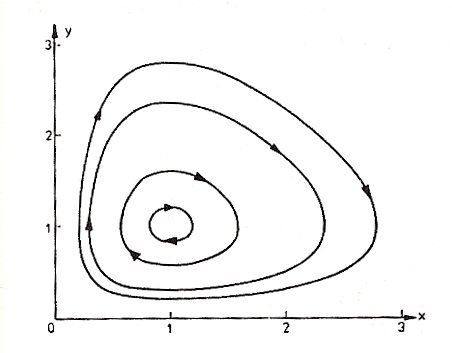
\includegraphics[width=\textwidth]{Bilder/Hamdyn.jpg}
\captionof{figure}{Dynamik des R"auber-Beute-Systems im Phasenraum}
\end{minipage}

\newpage
\section{Betrachtung mit der Master-Gleichung}
Es gibt zwei unterschiedliche Master-Gleichungen, welche prinzipiell das gegebene System beschreiben: zum einen ist das die diskrete Master-Gleichung
$$\frac{\partial}{\partial t} P(n, m, t)=k_1\,A (n-1) P(n-1, m, t) +k_{21}(n+1)(m-1) P(n+1, m-1, t)+k_2 (m+1) P(n, m+1, t)-$$ $$\left[ k_1 A n+ k_{21} n m +k_2 m \right] P(n,m,t)$$
bei welcher $n$ die Gr"o\ss e der Beute-Population und $m$ die der R"auber-Population ist. Diese ist jedoch nicht analytisch lösbar, da es hier zunächst unendlich viele miteinander gekoppelte Gleichungen gibt. Dieses Problem ist zwar durch die Einführung einer maximalen Populationsanzahl durchaus zu beheben, jedoch wird das System nicht handlicher, da bereits bei einer Maximalpopulation von 3 Tieren 10 gekoppelte Differentialgleichungen zu l"osen sind. Hier gelten  nun die Reaktionsgleichungen\\
$$x+A +e \xrightarrow{k_1} 2x $$
$$y \xrightarrow{k_2} e $$
$$x+y \xrightarrow[k_{21}]{k_{12}} y+y $$
dabei ist $e$ die Anzahl \glqq freier\grqq\ Plätze in dem System. Damit muss sich auch die erste Übergangsgröße verändern. Aus $k_1 A n$ wird nun $k_1 A n e$. Für den Kontinuitätsübergang werden nun noch die Größen  $x=\frac{n}{V}$, $y=\frac{m}{V}$ eingeführt.
Aber auch hier ist keine L"osung m"oglich, weshalb ein anderer L"osungsansatz ben"otigt wird. Im Folgenden soll dies mit Hilfe des Gillespie-Algorithmus' geschehen, welcher einen epirischen Ansatz verfolgt und das Problem numerisch l"osen kann.

\newpage
\section{Berechnungen mit dem Gillespie-Algorithmus}
Der Gillespie-Algorithmus untersucht stochastische Prozesse mit einem statistischen Ansatz: Es werden eine Anzahl von Durchl"aufen des Prozesses mit Hilfe von Zufallsfunktionen berechnet und anschließend "uber diese gemittelt. Wurden genügend Durchläufe gemacht und sind die verwendeten Zufallsalgorithmen gut, so entsprechen die mit dem Gillespie-Algorithmus gewonnenen Ergebnisse denen der analytische Lösung. Das genaue Vorgehen beim Gillespie-Algorithmus lautet wie folgt\footnote{http://www.co-nan.eu/pdf/df2.pdf (28.01.2013) }:
\begin{enumerate}
  \item Initialisiere zun"achst alle Startwerte (Anfangsbedingungen, Konstanten etc). In meiner Implementierung wird dieser Schritt separat bereits im constructor des Programms vorgenommen.
   \item Generiere zwei Zufallszahlen $\tau$, $\rho$, wobei $\tau$ eine exponentiell verteilte Zahl sein soll: Kleine Zahlen sollen also sehr häufig vorkommen, größere immer seltener (wird zum Beispiel, wie in meiner Implementierung, durch eine gleich-verteilte Zufallsvariable erzeugt, welche einer e-Funktion übergeben wird.). $\rho$ soll eine Zahl zwischen 0 und 1 sein. Die Werte von $\rho$ sind gleichverteilt (entsprechende Algorithmen bietet jede höhere Programmiersprache).\\
    In meiner Implementierung kommen keine Zeitsprünge größer als 1 Zeiteinheit vor:
         \begin{verbatim}
         double changetime=exp(-double(rand())/double(rand()))
         double reaction=double(rand())/RAND_MAX;\end{verbatim}
   \item Nun wird ein Reaktionsschritt durchgeführt: Die Zeit wird um die Variable $\tau$ weiter gesetzt (Zeitpunkt, zu dem die Reaktion stattfindet) und $\rho$ wird auf die möglichen Reaktionsschritte abgebildet. \\
   Da bei dem Räuber-Beute-Modell die Wahrscheinlichkeit von den Populationsgrößen abhängt, wird hier jeweils die Reaktionskonstante ($k_1$, $k_2$, $k_{21}$) mit der entsprechenden Populationsgröße addiert und durch die Gesamtgröße geteilt. In meiner Implementierung:
        \begin{verbatim}
         double foo=k1*prepre[i].prey[j];
         double bar=foo+k2*prepre[i].pred[j];
         double foobar=bar+(k21+k12)*prepre[i].pred[j]*prepre[i].prey[j]/2;
        \end{verbatim}
     Nun kann durch Vergleich der Größen einer der Prozesse durchgeführt werden:
        \begin{verbatim}
         if (reaction<=foo/foobar){ //a new  prey is born
         else if(reaction<=bar/foobar){ // a pred died
         else { //a pred ate a prey
        \end{verbatim}
   \item Ist die zu Beginn festgelegte Simulationsdauer noch nicht erreicht, beginne wieder bei Schritt 2. Dabei muss darauf geachtet werden, dass die Wahrscheinlichkeiten beim nächsten Reaktionsschritt anders verteilt sind.
\end{enumerate}
Die gesamte Implementierung des Algorithmus' kann auf der Seite

 \textbf{https://github.com/BalticPinguin/Prey-Predator-System.git} \\
eingesehen und heruntergeladen werden.

Mit Hilfe dieses Algorithmus' l"asst sich das R"auber-Beute-Modell nun gut beschreiben. Allerdings stellt sich die Suche nach geeigneten Parametern als deutlich schwerer dar, als man zunächst erwarten würde, da die Zusammenhänge, wie auch an den unten dargestellten Graphiken zu erkennen ist, nicht linear sind. Stirbt beispielsweise die Räuber-Population bei den Simulationen stets aus, hilft es nicht, ihr Sterberate einfach zu senken; vielmehr hilft ihnen eine höhere Geburtenzahl bei den Beutetieren, da sie sich so besser erholen und damit die Räuber-Population stärken.\\

\begin{minipage}[b]{0.58\textwidth} 
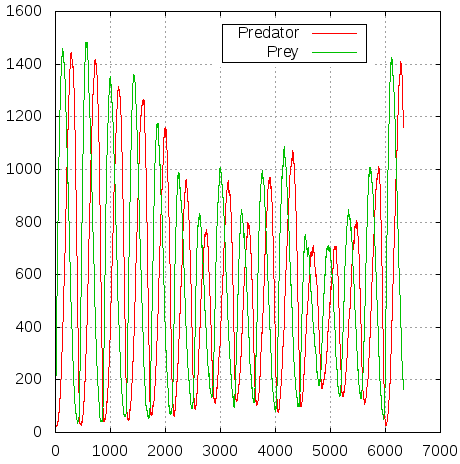
\includegraphics[width=\textwidth]{Graphiken/ppm1timepop.png}
\captionof{figure}{zeitliche Entwicklung der Populationen (Einzeltrajektorie)}
\end{minipage}
\hfill
\begin{minipage}[b]{0.39\textwidth}
Die nebenstehenden Graphiken zeigen eine mit dem Algorithmus berechnete Einzeltrajektorie; einmal als zeitlicher Verlauf (oben) und einmal im \glqq Phasenraum\grqq , welcher von den Populationgrößen aufgespannt wird. In diesem sieht man also die Kopplung der beiden Größen untereinander. 
Auch zeigt sich hier, abgesehen von dem spiralförmigen Verlauf, dass der berechnete Prozess offensichtlich dem oben betrachteten deterministischen Modell ähnlich ist, da die Prozesse in der gleichen leicht dreieckigen Form ablaufen.\\
Allerdings ist die hier abgebildete Trajektorie für die in diesem Prozess genutzten Parameter eher untypisch. Mittelt man hier über viele Prozesse, so zeigt sich, dass meist die Räuber-Population mehr oder weniger bald ausstirbt. Dadurch, dass es sich hier um eine Einzeltrajektorie handelt, sieht man hier aber sehr gut die stochastischen Schwankungen, denen der Zufallsprozess unterliegt.
\end{minipage}
\begin{minipage}[b]{0.58\textwidth}
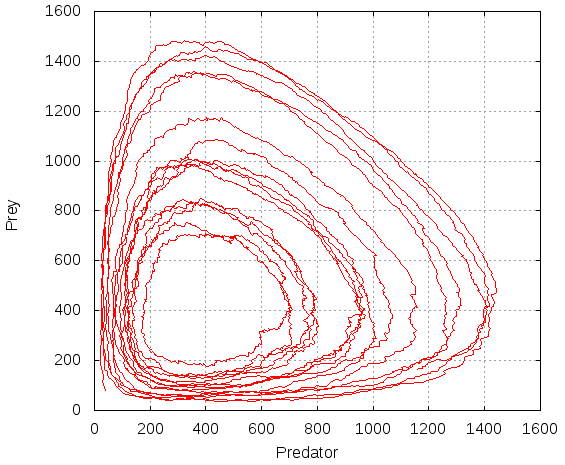
\includegraphics[width=\textwidth]{Graphiken/ppm1hampop.png}
\captionof{figure}{Entwicklung der beiden Populationen im Phasenraum (Einzeltrajektorie)}
\end{minipage}

\begin{minipage}[b]{0.58\textwidth}
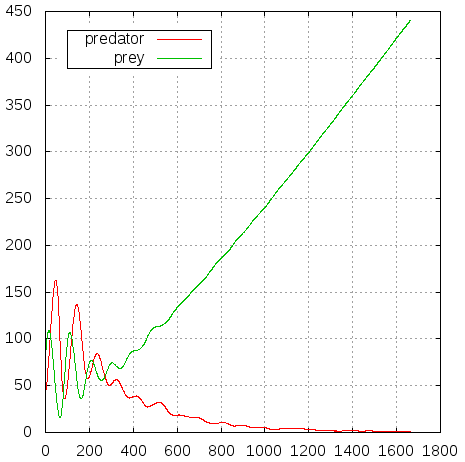
\includegraphics[width=\textwidth]{Graphiken/ppm42pop.png}
\captionof{figure}{zeitliche Populationsentwicklung, wenn R"auber-Population ausstirbt}
\end{minipage}
\hfil
\begin{minipage}[b]{0.39\textwidth}
Die hier abgebildeten Graphiken (oben zeitlicher Verlauf, unten Trajektorie im Phasenraum) entstanden aus einer Mittlung über 1000 Simulationsdurchläufe. Dabei wurden die Parameter hier so gewählt, dass sie die in der deterministischen Betrachtung oben gefundenen Bedingungen
$x=\frac{k_2}{k_{21}}$, $y=\frac{k_1\,A}{k_{12}}$\\
gen"ugen. Offensichtlich unterscheidet sich dieses Modell von dem deterministischen quantitativ recht stark. Die Parameter haben offensichtlich in diesem Modell doch eine etwas andere Bedeutung als in dem deterministischen Modell. Allerdings scheinen sie in ihrer Proportionalit"at denen oben zu entsprechen. So sind auch bei stabileren Durchl"aufen die Konstanten $k_{21}$ und $k_{12}$ um einige Gr"oßenodnungen kleiner als die anderen beiden. 
\end{minipage}
\begin{minipage}[b]{0.58\textwidth}
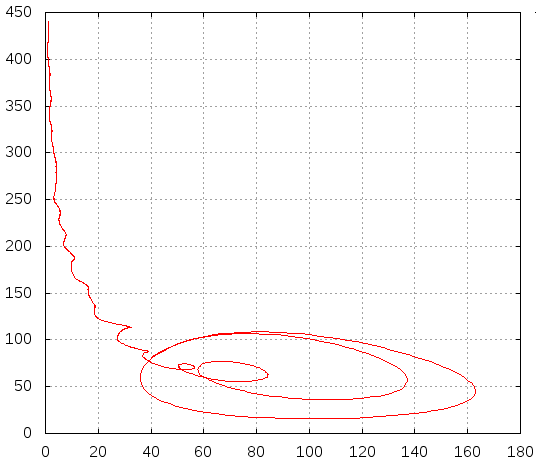
\includegraphics[width=\textwidth]{Graphiken/ppm42ham.png}
\captionof{figure}{obige Entwicklung im Phasenraum}
\end{minipage}

\begin{minipage}[b]{0.58\textwidth}
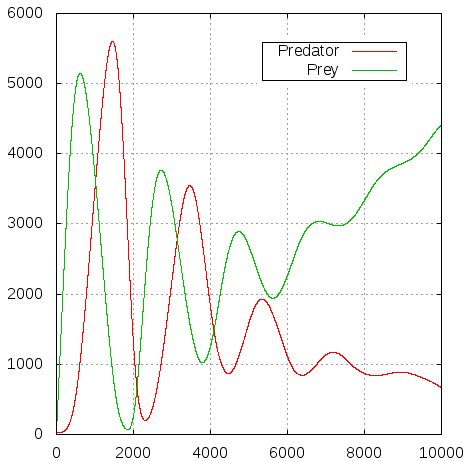
\includegraphics[width=1.0\textwidth]{Graphiken/ppm45pop.png}
\captionof{figure}{gemittelte Trajektorie in einem fast stabilen Zustand}
\end{minipage}
\begin{minipage}[b]{0.39\textwidth}
Wie die nebenstehenden Bilder zeigen, hat nicht nur die gewählte Auswertungsmethode, welche zu sehr großen Fehlern führt (welcher jedoch hier außerdem durch einen mittlerweile behobenen Fehler im Programm kommt), sondern auch zu keinen schönen Zyklen führt. Dies liegt vor allem an den Anfangsbedingungen\footnote{nature.berkeley.edu/biocon/BC Class Notes/ 73-77 Predator Models.pdf (am 07.08.2013)}, welche in vielen Fällen keine stabilen Zyklen erzeugen. Im Wesentlichen sind die Parameter offensichtlich so gew"ahlt, dass die R"auber-Population gegen Ende h"aufig ausstirbt, da die Beute-Population entsprechend ansteigt. Die Dämpfung wird jedoch, wie auch die Fehlerkurve nahelegt, vermutlich auch durch die Mittelung deutlich verstärkt.
\end{minipage}
\begin{minipage}[b]{0.48\textwidth}
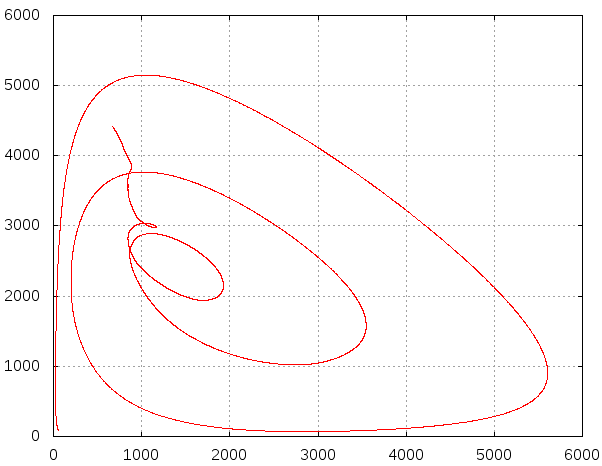
\includegraphics[width=1.0\textwidth]{Graphiken/ppm45ham.png}
\captionof{figure}{Trajektorie im Phasenraum}
\end{minipage}
\hfill
\begin{minipage}[b]{0.48\textwidth}
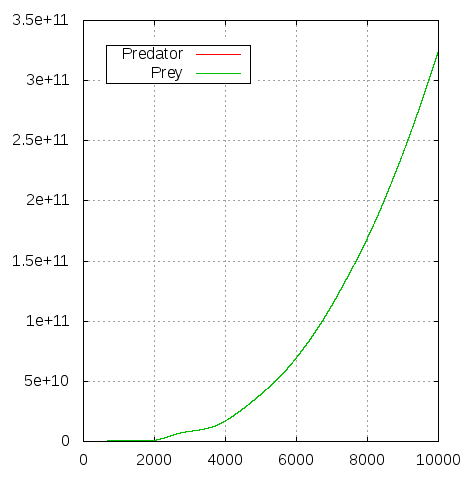
\includegraphics[width=1.0\textwidth]{Graphiken/ppm45abb.png}
\captionof{figure}{zeitliche Entwicklung der Standardabweichung im fast stabilen Zustand}
\end{minipage}

\hspace{5mm}

Weitere Beispiele für Simulationsdurchläufe sowie die jeweils genutzten Parameter können unter https://github.com/BalticPinguin/Prey-Predator-System im Odner \glqq Graphiken\grqq  heruntergeladen werden.

\section{Auswertung}
Das R"auber-Beute-Modell ist offensichtlich ein sehr ergibiges Problem, welches sich, wie die obigen Betrachtungen zeigen, auf verschiedene Weise beschreiben und untersuchen l"asst. Dabei hat jede Untersuchungsweise ihre Vor- und Nachteile; in der vorliegenden Arbeit konnte auch gezeigt werden, dass die beiden hier untersuchten Modelle einander doch recht ähnlich sind, da sie offensichtlich äquivalente Ergebnisse liefern. \\
Im Weiteren wären Untersuchungen über die genauen Einflüsse der Parameter sowie Stabilisierungsversuche sehr interessant, da diese weiteren Aufschluss über das System geben würden. Im Rahmen dieser Arbeit musste darauf verzichtet werden, da dies einigen Aufwand mit sich bringen würde und bei der vorliegenden Implementierung wohl allgemein zu aufwändig wäre. Die Suche nach geeigneten Parametern für eine langfristig stabile Simulation hat mir jedoch bereits gezeigt, dass diese Zusammenhänge recht komplex zu sein scheinen, was ihre Untersuchung um so interessanter gestalten würde.\\

\section{Abbildungsverzeichnis}
\begin{itemize}
   \item Quellen Titelbild: http://iqa.evergreenps.org/science/biology/predator-prey\_files/pred-prey.jpg (13.02.2013),\\
        http://www.globalchange.umich.edu/globalchange1/current/lectures/predation/tmp26.gif (04.01.2013)
   \item Abbildung 1: R. Mahnke \glqq Nichtlineare Physik in Aufgaben \grqq Verlag: B.G. Teubner, Stuttgart 1994; S. 125
   \item Abbildung 2-3: Parameter: 80, 40, 6500, 4.8, 2.0, 0.01, 0,01, 1
   \item Abbildung 4-5: Parameter: 80, 40, 1700, 5.6, 2.8, 0.07, 0.07, 1000
   \item Abbildung 6-8: Parameter: 80, 60, 50000, 11.2, 8.1, 0.011, 0.011, 1000
\end{itemize}
\textit{Hinweis zu der Parameterangabe: Reihenfolge der angegebenen Zahlen:\\
 Beutepopulation, R"auber-Population (jew. Startwerte) , zu durchlaufende Zeiteinheiten, $k_1\,A$, $k_2$, $k_{21}$, $k_{12}$, Anzahl der berechneten Simulationen}
\end{document}
